% Options for packages loaded elsewhere
\PassOptionsToPackage{unicode}{hyperref}
\PassOptionsToPackage{hyphens}{url}
%
\documentclass[
]{article}
\usepackage{amsmath,amssymb}
\usepackage{lmodern}
\usepackage{ifxetex,ifluatex}
\ifnum 0\ifxetex 1\fi\ifluatex 1\fi=0 % if pdftex
  \usepackage[T1]{fontenc}
  \usepackage[utf8]{inputenc}
  \usepackage{textcomp} % provide euro and other symbols
\else % if luatex or xetex
  \usepackage{unicode-math}
  \defaultfontfeatures{Scale=MatchLowercase}
  \defaultfontfeatures[\rmfamily]{Ligatures=TeX,Scale=1}
\fi
% Use upquote if available, for straight quotes in verbatim environments
\IfFileExists{upquote.sty}{\usepackage{upquote}}{}
\IfFileExists{microtype.sty}{% use microtype if available
  \usepackage[]{microtype}
  \UseMicrotypeSet[protrusion]{basicmath} % disable protrusion for tt fonts
}{}
\makeatletter
\@ifundefined{KOMAClassName}{% if non-KOMA class
  \IfFileExists{parskip.sty}{%
    \usepackage{parskip}
  }{% else
    \setlength{\parindent}{0pt}
    \setlength{\parskip}{6pt plus 2pt minus 1pt}}
}{% if KOMA class
  \KOMAoptions{parskip=half}}
\makeatother
\usepackage{xcolor}
\IfFileExists{xurl.sty}{\usepackage{xurl}}{} % add URL line breaks if available
\IfFileExists{bookmark.sty}{\usepackage{bookmark}}{\usepackage{hyperref}}
\hypersetup{
  pdftitle={p8105\_hw6\_fs2757},
  pdfauthor={FEI SUN},
  hidelinks,
  pdfcreator={LaTeX via pandoc}}
\urlstyle{same} % disable monospaced font for URLs
\usepackage[margin=1in]{geometry}
\usepackage{color}
\usepackage{fancyvrb}
\newcommand{\VerbBar}{|}
\newcommand{\VERB}{\Verb[commandchars=\\\{\}]}
\DefineVerbatimEnvironment{Highlighting}{Verbatim}{commandchars=\\\{\}}
% Add ',fontsize=\small' for more characters per line
\usepackage{framed}
\definecolor{shadecolor}{RGB}{248,248,248}
\newenvironment{Shaded}{\begin{snugshade}}{\end{snugshade}}
\newcommand{\AlertTok}[1]{\textcolor[rgb]{0.94,0.16,0.16}{#1}}
\newcommand{\AnnotationTok}[1]{\textcolor[rgb]{0.56,0.35,0.01}{\textbf{\textit{#1}}}}
\newcommand{\AttributeTok}[1]{\textcolor[rgb]{0.77,0.63,0.00}{#1}}
\newcommand{\BaseNTok}[1]{\textcolor[rgb]{0.00,0.00,0.81}{#1}}
\newcommand{\BuiltInTok}[1]{#1}
\newcommand{\CharTok}[1]{\textcolor[rgb]{0.31,0.60,0.02}{#1}}
\newcommand{\CommentTok}[1]{\textcolor[rgb]{0.56,0.35,0.01}{\textit{#1}}}
\newcommand{\CommentVarTok}[1]{\textcolor[rgb]{0.56,0.35,0.01}{\textbf{\textit{#1}}}}
\newcommand{\ConstantTok}[1]{\textcolor[rgb]{0.00,0.00,0.00}{#1}}
\newcommand{\ControlFlowTok}[1]{\textcolor[rgb]{0.13,0.29,0.53}{\textbf{#1}}}
\newcommand{\DataTypeTok}[1]{\textcolor[rgb]{0.13,0.29,0.53}{#1}}
\newcommand{\DecValTok}[1]{\textcolor[rgb]{0.00,0.00,0.81}{#1}}
\newcommand{\DocumentationTok}[1]{\textcolor[rgb]{0.56,0.35,0.01}{\textbf{\textit{#1}}}}
\newcommand{\ErrorTok}[1]{\textcolor[rgb]{0.64,0.00,0.00}{\textbf{#1}}}
\newcommand{\ExtensionTok}[1]{#1}
\newcommand{\FloatTok}[1]{\textcolor[rgb]{0.00,0.00,0.81}{#1}}
\newcommand{\FunctionTok}[1]{\textcolor[rgb]{0.00,0.00,0.00}{#1}}
\newcommand{\ImportTok}[1]{#1}
\newcommand{\InformationTok}[1]{\textcolor[rgb]{0.56,0.35,0.01}{\textbf{\textit{#1}}}}
\newcommand{\KeywordTok}[1]{\textcolor[rgb]{0.13,0.29,0.53}{\textbf{#1}}}
\newcommand{\NormalTok}[1]{#1}
\newcommand{\OperatorTok}[1]{\textcolor[rgb]{0.81,0.36,0.00}{\textbf{#1}}}
\newcommand{\OtherTok}[1]{\textcolor[rgb]{0.56,0.35,0.01}{#1}}
\newcommand{\PreprocessorTok}[1]{\textcolor[rgb]{0.56,0.35,0.01}{\textit{#1}}}
\newcommand{\RegionMarkerTok}[1]{#1}
\newcommand{\SpecialCharTok}[1]{\textcolor[rgb]{0.00,0.00,0.00}{#1}}
\newcommand{\SpecialStringTok}[1]{\textcolor[rgb]{0.31,0.60,0.02}{#1}}
\newcommand{\StringTok}[1]{\textcolor[rgb]{0.31,0.60,0.02}{#1}}
\newcommand{\VariableTok}[1]{\textcolor[rgb]{0.00,0.00,0.00}{#1}}
\newcommand{\VerbatimStringTok}[1]{\textcolor[rgb]{0.31,0.60,0.02}{#1}}
\newcommand{\WarningTok}[1]{\textcolor[rgb]{0.56,0.35,0.01}{\textbf{\textit{#1}}}}
\usepackage{longtable,booktabs,array}
\usepackage{calc} % for calculating minipage widths
% Correct order of tables after \paragraph or \subparagraph
\usepackage{etoolbox}
\makeatletter
\patchcmd\longtable{\par}{\if@noskipsec\mbox{}\fi\par}{}{}
\makeatother
% Allow footnotes in longtable head/foot
\IfFileExists{footnotehyper.sty}{\usepackage{footnotehyper}}{\usepackage{footnote}}
\makesavenoteenv{longtable}
\usepackage{graphicx}
\makeatletter
\def\maxwidth{\ifdim\Gin@nat@width>\linewidth\linewidth\else\Gin@nat@width\fi}
\def\maxheight{\ifdim\Gin@nat@height>\textheight\textheight\else\Gin@nat@height\fi}
\makeatother
% Scale images if necessary, so that they will not overflow the page
% margins by default, and it is still possible to overwrite the defaults
% using explicit options in \includegraphics[width, height, ...]{}
\setkeys{Gin}{width=\maxwidth,height=\maxheight,keepaspectratio}
% Set default figure placement to htbp
\makeatletter
\def\fps@figure{htbp}
\makeatother
\setlength{\emergencystretch}{3em} % prevent overfull lines
\providecommand{\tightlist}{%
  \setlength{\itemsep}{0pt}\setlength{\parskip}{0pt}}
\setcounter{secnumdepth}{-\maxdimen} % remove section numbering
\ifluatex
  \usepackage{selnolig}  % disable illegal ligatures
\fi

\title{p8105\_hw6\_fs2757}
\author{FEI SUN}
\date{2021/12/2}

\begin{document}
\maketitle

\hypertarget{problem-1}{%
\section{Problem 1}\label{problem-1}}

\begin{Shaded}
\begin{Highlighting}[]
\NormalTok{birthweight\_raw }\OtherTok{=} 
  \FunctionTok{read\_csv}\NormalTok{(}\StringTok{"data/birthweight.csv"}\NormalTok{) }\SpecialCharTok{\%\textgreater{}\%} 
\NormalTok{  janitor}\SpecialCharTok{::}\FunctionTok{clean\_names}\NormalTok{()}\SpecialCharTok{\%\textgreater{}\%} 
  \FunctionTok{mutate}\NormalTok{(}
    \AttributeTok{babysex =} \FunctionTok{case\_when}\NormalTok{(babysex }\SpecialCharTok{==} \StringTok{"1"} \SpecialCharTok{\textasciitilde{}} \StringTok{"male"}\NormalTok{,}
\NormalTok{                        babysex }\SpecialCharTok{==} \StringTok{"2"} \SpecialCharTok{\textasciitilde{}} \StringTok{"female"}\NormalTok{),}
    \AttributeTok{frace =} \FunctionTok{case\_when}\NormalTok{(frace }\SpecialCharTok{==} \StringTok{"1"} \SpecialCharTok{\textasciitilde{}} \StringTok{"White"}\NormalTok{,}
\NormalTok{                      frace }\SpecialCharTok{==} \StringTok{"2"} \SpecialCharTok{\textasciitilde{}} \StringTok{"Black"}\NormalTok{,}
\NormalTok{                      frace }\SpecialCharTok{==} \StringTok{"3"} \SpecialCharTok{\textasciitilde{}} \StringTok{"Asian"}\NormalTok{,}
\NormalTok{                      frace }\SpecialCharTok{==} \StringTok{"4"} \SpecialCharTok{\textasciitilde{}} \StringTok{"Puerto Rican"}\NormalTok{, }
\NormalTok{                      frace }\SpecialCharTok{==} \StringTok{"8"} \SpecialCharTok{\textasciitilde{}} \StringTok{"Other"}\NormalTok{,}
\NormalTok{                      frace }\SpecialCharTok{==} \StringTok{"9"} \SpecialCharTok{\textasciitilde{}} \StringTok{"Unknown"}\NormalTok{),}
    \AttributeTok{malform =} \FunctionTok{case\_when}\NormalTok{(malform }\SpecialCharTok{==} \StringTok{"0"} \SpecialCharTok{\textasciitilde{}} \StringTok{"absent"}\NormalTok{,}
\NormalTok{                        malform }\SpecialCharTok{==} \StringTok{"1"} \SpecialCharTok{\textasciitilde{}} \StringTok{"present"}\NormalTok{),}
    \AttributeTok{mrace =} \FunctionTok{case\_when}\NormalTok{(mrace }\SpecialCharTok{==} \StringTok{"1"} \SpecialCharTok{\textasciitilde{}} \StringTok{"White"}\NormalTok{,}
\NormalTok{                      mrace }\SpecialCharTok{==} \StringTok{"2"} \SpecialCharTok{\textasciitilde{}} \StringTok{"Black"}\NormalTok{,}
\NormalTok{                      mrace }\SpecialCharTok{==} \StringTok{"3"} \SpecialCharTok{\textasciitilde{}} \StringTok{"Asian"}\NormalTok{,}
\NormalTok{                      mrace }\SpecialCharTok{==} \StringTok{"4"} \SpecialCharTok{\textasciitilde{}} \StringTok{"Puerto Rican"}\NormalTok{,}
\NormalTok{                      mrace }\SpecialCharTok{==} \StringTok{"8"} \SpecialCharTok{\textasciitilde{}} \StringTok{"Other"}\NormalTok{),}
    \AttributeTok{babysex =} \FunctionTok{as.factor}\NormalTok{(babysex),}
    \AttributeTok{frace =} \FunctionTok{as.factor}\NormalTok{(frace),}
    \AttributeTok{malform =} \FunctionTok{as.factor}\NormalTok{(malform),}
    \AttributeTok{mrace =} \FunctionTok{as.factor}\NormalTok{(mrace))}
\end{Highlighting}
\end{Shaded}

\begin{verbatim}
## Rows: 4342 Columns: 20
\end{verbatim}

\begin{verbatim}
## -- Column specification --------------------------------------------------------
## Delimiter: ","
## dbl (20): babysex, bhead, blength, bwt, delwt, fincome, frace, gaweeks, malf...
\end{verbatim}

\begin{verbatim}
## 
## i Use `spec()` to retrieve the full column specification for this data.
## i Specify the column types or set `show_col_types = FALSE` to quiet this message.
\end{verbatim}

\begin{Shaded}
\begin{Highlighting}[]
\NormalTok{skimr}\SpecialCharTok{::}\FunctionTok{skim}\NormalTok{(birthweight\_raw)}
\end{Highlighting}
\end{Shaded}

\begin{longtable}[]{@{}ll@{}}
\caption{Data summary}\tabularnewline
\toprule
& \\
\midrule
\endfirsthead
\toprule
& \\
\midrule
\endhead
Name & birthweight\_raw \\
Number of rows & 4342 \\
Number of columns & 20 \\
\_\_\_\_\_\_\_\_\_\_\_\_\_\_\_\_\_\_\_\_\_\_\_ & \\
Column type frequency: & \\
factor & 4 \\
numeric & 16 \\
\_\_\_\_\_\_\_\_\_\_\_\_\_\_\_\_\_\_\_\_\_\_\_\_ & \\
Group variables & None \\
\bottomrule
\end{longtable}

\textbf{Variable type: factor}

\begin{longtable}[]{@{}lrrlrl@{}}
\toprule
skim\_variable & n\_missing & complete\_rate & ordered & n\_unique &
top\_counts \\
\midrule
\endhead
babysex & 0 & 1 & FALSE & 2 & mal: 2230, fem: 2112 \\
frace & 0 & 1 & FALSE & 5 & Whi: 2123, Bla: 1911, Pue: 248, Asi: 46 \\
malform & 0 & 1 & FALSE & 2 & abs: 4327, pre: 15 \\
mrace & 0 & 1 & FALSE & 4 & Whi: 2147, Bla: 1909, Pue: 243, Asi: 43 \\
\bottomrule
\end{longtable}

\textbf{Variable type: numeric}

\begin{longtable}[]{@{}lrrrrrrrrrl@{}}
\toprule
skim\_variable & n\_missing & complete\_rate & mean & sd & p0 & p25 &
p50 & p75 & p100 & hist \\
\midrule
\endhead
bhead & 0 & 1 & 33.65 & 1.62 & 21.00 & 33.00 & 34.00 & 35.00 & 41.0 &
▁▁▆▇▁ \\
blength & 0 & 1 & 49.75 & 2.72 & 20.00 & 48.00 & 50.00 & 51.00 & 63.0 &
▁▁▁▇▁ \\
bwt & 0 & 1 & 3114.40 & 512.15 & 595.00 & 2807.00 & 3132.50 & 3459.00 &
4791.0 & ▁▁▇▇▁ \\
delwt & 0 & 1 & 145.57 & 22.21 & 86.00 & 131.00 & 143.00 & 157.00 &
334.0 & ▅▇▁▁▁ \\
fincome & 0 & 1 & 44.11 & 25.98 & 0.00 & 25.00 & 35.00 & 65.00 & 96.0 &
▃▇▅▂▃ \\
gaweeks & 0 & 1 & 39.43 & 3.15 & 17.70 & 38.30 & 39.90 & 41.10 & 51.3 &
▁▁▂▇▁ \\
menarche & 0 & 1 & 12.51 & 1.48 & 0.00 & 12.00 & 12.00 & 13.00 & 19.0 &
▁▁▂▇▁ \\
mheight & 0 & 1 & 63.49 & 2.66 & 48.00 & 62.00 & 63.00 & 65.00 & 77.0 &
▁▁▇▂▁ \\
momage & 0 & 1 & 20.30 & 3.88 & 12.00 & 18.00 & 20.00 & 22.00 & 44.0 &
▅▇▂▁▁ \\
parity & 0 & 1 & 0.00 & 0.10 & 0.00 & 0.00 & 0.00 & 0.00 & 6.0 &
▇▁▁▁▁ \\
pnumlbw & 0 & 1 & 0.00 & 0.00 & 0.00 & 0.00 & 0.00 & 0.00 & 0.0 &
▁▁▇▁▁ \\
pnumsga & 0 & 1 & 0.00 & 0.00 & 0.00 & 0.00 & 0.00 & 0.00 & 0.0 &
▁▁▇▁▁ \\
ppbmi & 0 & 1 & 21.57 & 3.18 & 13.07 & 19.53 & 21.03 & 22.91 & 46.1 &
▃▇▁▁▁ \\
ppwt & 0 & 1 & 123.49 & 20.16 & 70.00 & 110.00 & 120.00 & 134.00 & 287.0
& ▅▇▁▁▁ \\
smoken & 0 & 1 & 4.15 & 7.41 & 0.00 & 0.00 & 0.00 & 5.00 & 60.0 &
▇▁▁▁▁ \\
wtgain & 0 & 1 & 22.08 & 10.94 & -46.00 & 15.00 & 22.00 & 28.00 & 89.0 &
▁▁▇▁▁ \\
\bottomrule
\end{longtable}

There are no missing value in the dataset. Also I convert the numeric
variable to the factor.

\begin{Shaded}
\begin{Highlighting}[]
\NormalTok{model1 }\OtherTok{=} \FunctionTok{lm}\NormalTok{(bwt }\SpecialCharTok{\textasciitilde{}}\NormalTok{gaweeks }\SpecialCharTok{+}\NormalTok{ babysex }\SpecialCharTok{+}\NormalTok{ mheight }\SpecialCharTok{+}\NormalTok{ ppwt }\SpecialCharTok{+}\NormalTok{ wtgain }\SpecialCharTok{+}\NormalTok{ parity }\SpecialCharTok{+}\NormalTok{ smoken }\SpecialCharTok{+}\NormalTok{ bhead }\SpecialCharTok{+}\NormalTok{ mrace }\SpecialCharTok{+}\NormalTok{ frace }\SpecialCharTok{+}\NormalTok{ malform, }\AttributeTok{data =}\NormalTok{ birthweight\_raw)}
\FunctionTok{summary}\NormalTok{(model1)}
\end{Highlighting}
\end{Shaded}

\begin{verbatim}
## 
## Call:
## lm(formula = bwt ~ gaweeks + babysex + mheight + ppwt + wtgain + 
##     parity + smoken + bhead + mrace + frace + malform, data = birthweight_raw)
## 
## Residuals:
##      Min       1Q   Median       3Q      Max 
## -1088.43  -211.58    -1.68   204.37  2173.25 
## 
## Coefficients:
##                     Estimate Std. Error t value Pr(>|t|)    
## (Intercept)       -5381.3983   161.8347 -33.252  < 2e-16 ***
## gaweeks              19.9606     1.6587  12.034  < 2e-16 ***
## babysexmale         -22.0134     9.7093  -2.267   0.0234 *  
## mheight              11.4697     2.0394   5.624 1.98e-08 ***
## ppwt                  1.9527     0.2663   7.332 2.68e-13 ***
## wtgain                5.4998     0.4484  12.266  < 2e-16 ***
## parity               74.2742    46.3118   1.604   0.1088    
## smoken               -6.7193     0.6710 -10.013  < 2e-16 ***
## bhead               198.0515     3.3685  58.795  < 2e-16 ***
## mraceBlack          -56.0018    92.6802  -0.604   0.5457    
## mracePuerto Rican     9.2377    92.6871   0.100   0.9206    
## mraceWhite          103.8208    82.3966   1.260   0.2077    
## fraceBlack          -41.2463    90.4087  -0.456   0.6483    
## fraceOther          -57.0841   111.9218  -0.510   0.6101    
## fracePuerto Rican   -62.2455    90.0432  -0.691   0.4894    
## fraceWhite          -26.2586    79.4810  -0.330   0.7411    
## malformpresent      -31.3401    81.0268  -0.387   0.6989    
## ---
## Signif. codes:  0 '***' 0.001 '**' 0.01 '*' 0.05 '.' 0.1 ' ' 1
## 
## Residual standard error: 312.8 on 4325 degrees of freedom
## Multiple R-squared:  0.6284, Adjusted R-squared:  0.6271 
## F-statistic: 457.2 on 16 and 4325 DF,  p-value: < 2.2e-16
\end{verbatim}

\begin{Shaded}
\begin{Highlighting}[]
\NormalTok{broom}\SpecialCharTok{::}\FunctionTok{tidy}\NormalTok{(model1)}
\end{Highlighting}
\end{Shaded}

\begin{verbatim}
## # A tibble: 17 x 5
##    term              estimate std.error statistic   p.value
##    <chr>                <dbl>     <dbl>     <dbl>     <dbl>
##  1 (Intercept)       -5381.     162.     -33.3    4.16e-216
##  2 gaweeks              20.0      1.66    12.0    7.84e- 33
##  3 babysexmale         -22.0      9.71    -2.27   2.34e-  2
##  4 mheight              11.5      2.04     5.62   1.98e-  8
##  5 ppwt                  1.95     0.266    7.33   2.68e- 13
##  6 wtgain                5.50     0.448   12.3    5.02e- 34
##  7 parity               74.3     46.3      1.60   1.09e-  1
##  8 smoken               -6.72     0.671  -10.0    2.39e- 23
##  9 bhead               198.       3.37    58.8    0        
## 10 mraceBlack          -56.0     92.7     -0.604  5.46e-  1
## 11 mracePuerto Rican     9.24    92.7      0.0997 9.21e-  1
## 12 mraceWhite          104.      82.4      1.26   2.08e-  1
## 13 fraceBlack          -41.2     90.4     -0.456  6.48e-  1
## 14 fraceOther          -57.1    112.      -0.510  6.10e-  1
## 15 fracePuerto Rican   -62.2     90.0     -0.691  4.89e-  1
## 16 fraceWhite          -26.3     79.5     -0.330  7.41e-  1
## 17 malformpresent      -31.3     81.0     -0.387  6.99e-  1
\end{verbatim}

\begin{Shaded}
\begin{Highlighting}[]
\NormalTok{birthweight\_raw }\SpecialCharTok{\%\textgreater{}\%} 
\NormalTok{  modelr}\SpecialCharTok{::}\FunctionTok{add\_residuals}\NormalTok{(model1) }\SpecialCharTok{\%\textgreater{}\%} 
\NormalTok{  modelr}\SpecialCharTok{::}\FunctionTok{add\_predictions}\NormalTok{(model1) }\SpecialCharTok{\%\textgreater{}\%} 
  \FunctionTok{ggplot}\NormalTok{(}\FunctionTok{aes}\NormalTok{(}\AttributeTok{x =}\NormalTok{ pred, }\AttributeTok{y =}\NormalTok{ resid,}\AttributeTok{color=}\NormalTok{babysex))}\SpecialCharTok{+}
  \FunctionTok{geom\_point}\NormalTok{(}\AttributeTok{alpha =} \FloatTok{0.3}\NormalTok{)}\SpecialCharTok{+}
  \FunctionTok{geom\_smooth}\NormalTok{(}\AttributeTok{color =} \StringTok{"green"}\NormalTok{,}\AttributeTok{method =} \StringTok{"lm"}\NormalTok{, }\AttributeTok{se =}\NormalTok{ F)}\SpecialCharTok{+}
  \FunctionTok{facet\_grid}\NormalTok{(. }\SpecialCharTok{\textasciitilde{}}\NormalTok{ babysex)}\SpecialCharTok{+}
  \FunctionTok{labs}\NormalTok{(}
    \AttributeTok{x =} \StringTok{"Fitted Value"}\NormalTok{,}
    \AttributeTok{y =} \StringTok{"Residuals"}\NormalTok{,}
    \AttributeTok{title =} \StringTok{"Plot of Residuals against Fitted Value"}
\NormalTok{  )}
\end{Highlighting}
\end{Shaded}

\begin{verbatim}
## `geom_smooth()` using formula 'y ~ x'
\end{verbatim}

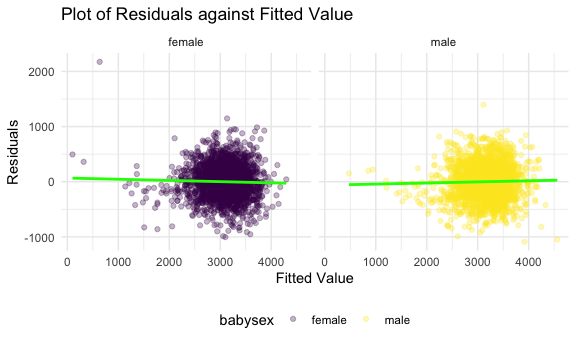
\includegraphics[width=0.9\linewidth]{p8105_hw6_fs2757_files/figure-latex/unnamed-chunk-2-1}

About model 1, I will using almost all clinically relevant variables as
predictors(X) based on current literature and removed all
non-significant predictors. From the plot, it shows that the residuals
are relatively evenly distributed around y = 0 and it satisfies the
linearity assumption.

\begin{Shaded}
\begin{Highlighting}[]
\NormalTok{model2 }\OtherTok{=} \FunctionTok{lm}\NormalTok{(bwt }\SpecialCharTok{\textasciitilde{}}\NormalTok{blength }\SpecialCharTok{+}\NormalTok{ gaweeks, }\AttributeTok{data =}\NormalTok{ birthweight\_raw)}
\FunctionTok{summary}\NormalTok{(model2)}
\end{Highlighting}
\end{Shaded}

\begin{verbatim}
## 
## Call:
## lm(formula = bwt ~ blength + gaweeks, data = birthweight_raw)
## 
## Residuals:
##     Min      1Q  Median      3Q     Max 
## -1709.6  -215.4   -11.4   208.2  4188.8 
## 
## Coefficients:
##              Estimate Std. Error t value Pr(>|t|)    
## (Intercept) -4347.667     97.958  -44.38   <2e-16 ***
## blength       128.556      1.990   64.60   <2e-16 ***
## gaweeks        27.047      1.718   15.74   <2e-16 ***
## ---
## Signif. codes:  0 '***' 0.001 '**' 0.01 '*' 0.05 '.' 0.1 ' ' 1
## 
## Residual standard error: 333.2 on 4339 degrees of freedom
## Multiple R-squared:  0.5769, Adjusted R-squared:  0.5767 
## F-statistic:  2958 on 2 and 4339 DF,  p-value: < 2.2e-16
\end{verbatim}

\begin{Shaded}
\begin{Highlighting}[]
\NormalTok{broom}\SpecialCharTok{::}\FunctionTok{tidy}\NormalTok{(model2)}
\end{Highlighting}
\end{Shaded}

\begin{verbatim}
## # A tibble: 3 x 5
##   term        estimate std.error statistic  p.value
##   <chr>          <dbl>     <dbl>     <dbl>    <dbl>
## 1 (Intercept)  -4348.      98.0      -44.4 0       
## 2 blength        129.       1.99      64.6 0       
## 3 gaweeks         27.0      1.72      15.7 2.36e-54
\end{verbatim}

\begin{Shaded}
\begin{Highlighting}[]
\NormalTok{model3 }\OtherTok{=} \FunctionTok{lm}\NormalTok{(bwt }\SpecialCharTok{\textasciitilde{}}\NormalTok{bhead }\SpecialCharTok{+}\NormalTok{ blength }\SpecialCharTok{+}\NormalTok{ babysex }\SpecialCharTok{+} 
\NormalTok{              bhead }\SpecialCharTok{*}\NormalTok{ blength }\SpecialCharTok{+}\NormalTok{ bhead }\SpecialCharTok{*}\NormalTok{ babysex }\SpecialCharTok{+}\NormalTok{ blength }\SpecialCharTok{*}\NormalTok{ babysex }\SpecialCharTok{+}\NormalTok{ bhead }\SpecialCharTok{*}\NormalTok{ blength }\SpecialCharTok{*}\NormalTok{ babysex, }\AttributeTok{data =}\NormalTok{ birthweight\_raw)}
\FunctionTok{summary}\NormalTok{(model3)}
\end{Highlighting}
\end{Shaded}

\begin{verbatim}
## 
## Call:
## lm(formula = bwt ~ bhead + blength + babysex + bhead * blength + 
##     bhead * babysex + blength * babysex + bhead * blength * babysex, 
##     data = birthweight_raw)
## 
## Residuals:
##      Min       1Q   Median       3Q      Max 
## -1132.99  -190.42   -10.33   178.63  2617.96 
## 
## Coefficients:
##                             Estimate Std. Error t value Pr(>|t|)    
## (Intercept)                -801.9487  1102.3077  -0.728 0.466948    
## bhead                       -16.5975    34.0916  -0.487 0.626388    
## blength                     -21.6460    23.3720  -0.926 0.354421    
## babysexmale               -6374.8684  1677.7669  -3.800 0.000147 ***
## bhead:blength                 3.3244     0.7126   4.666 3.17e-06 ***
## bhead:babysexmale           198.3932    51.0917   3.883 0.000105 ***
## blength:babysexmale         123.7729    35.1185   3.524 0.000429 ***
## bhead:blength:babysexmale    -3.8781     1.0566  -3.670 0.000245 ***
## ---
## Signif. codes:  0 '***' 0.001 '**' 0.01 '*' 0.05 '.' 0.1 ' ' 1
## 
## Residual standard error: 287.7 on 4334 degrees of freedom
## Multiple R-squared:  0.6849, Adjusted R-squared:  0.6844 
## F-statistic:  1346 on 7 and 4334 DF,  p-value: < 2.2e-16
\end{verbatim}

\begin{Shaded}
\begin{Highlighting}[]
\NormalTok{broom}\SpecialCharTok{::}\FunctionTok{tidy}\NormalTok{(model3)}
\end{Highlighting}
\end{Shaded}

\begin{verbatim}
## # A tibble: 8 x 5
##   term                      estimate std.error statistic    p.value
##   <chr>                        <dbl>     <dbl>     <dbl>      <dbl>
## 1 (Intercept)                -802.    1102.       -0.728 0.467     
## 2 bhead                       -16.6     34.1      -0.487 0.626     
## 3 blength                     -21.6     23.4      -0.926 0.354     
## 4 babysexmale               -6375.    1678.       -3.80  0.000147  
## 5 bhead:blength                 3.32     0.713     4.67  0.00000317
## 6 bhead:babysexmale           198.      51.1       3.88  0.000105  
## 7 blength:babysexmale         124.      35.1       3.52  0.000429  
## 8 bhead:blength:babysexmale    -3.88     1.06     -3.67  0.000245
\end{verbatim}

\begin{Shaded}
\begin{Highlighting}[]
\NormalTok{cv\_df }\OtherTok{=}
  \FunctionTok{crossv\_mc}\NormalTok{(birthweight\_raw, }\DecValTok{100}\NormalTok{) }\SpecialCharTok{\%\textgreater{}\%}
  \FunctionTok{mutate}\NormalTok{(}
    \AttributeTok{train =} \FunctionTok{map}\NormalTok{(train, as\_tibble),}
    \AttributeTok{test =} \FunctionTok{map}\NormalTok{(test, as\_tibble))}\SpecialCharTok{\%\textgreater{}\%}
  \FunctionTok{mutate}\NormalTok{(}
    \AttributeTok{model\_1  =} \FunctionTok{map}\NormalTok{(train, }\SpecialCharTok{\textasciitilde{}}\FunctionTok{lm}\NormalTok{(bwt }\SpecialCharTok{\textasciitilde{}}\NormalTok{babysex }\SpecialCharTok{+}\NormalTok{ bhead }\SpecialCharTok{+}\NormalTok{ blength }\SpecialCharTok{+}\NormalTok{ delwt }\SpecialCharTok{+}\NormalTok{ fincome, }\AttributeTok{data =}\NormalTok{ .x)),}
    \AttributeTok{model\_2  =} \FunctionTok{map}\NormalTok{(train, }\SpecialCharTok{\textasciitilde{}}\FunctionTok{lm}\NormalTok{(bwt }\SpecialCharTok{\textasciitilde{}}\NormalTok{blength }\SpecialCharTok{+}\NormalTok{ gaweeks, }\AttributeTok{data =}\NormalTok{ .x)),}
    \AttributeTok{model\_3  =} \FunctionTok{map}\NormalTok{(train, }\SpecialCharTok{\textasciitilde{}}\FunctionTok{lm}\NormalTok{(bwt }\SpecialCharTok{\textasciitilde{}}\NormalTok{bhead }\SpecialCharTok{+}\NormalTok{ blength }\SpecialCharTok{+}\NormalTok{ babysex }\SpecialCharTok{+} 
\NormalTok{              bhead }\SpecialCharTok{*}\NormalTok{ blength }\SpecialCharTok{+}\NormalTok{ bhead }\SpecialCharTok{*}\NormalTok{ babysex }\SpecialCharTok{+}\NormalTok{ blength }\SpecialCharTok{*}\NormalTok{ babysex }\SpecialCharTok{+}\NormalTok{ bhead }\SpecialCharTok{*}\NormalTok{ blength }\SpecialCharTok{*}\NormalTok{ babysex,}
              \AttributeTok{data =}\NormalTok{ .x))) }\SpecialCharTok{\%\textgreater{}\%} 
  \FunctionTok{mutate}\NormalTok{(}\AttributeTok{rmse\_model1 =} 
        \FunctionTok{map2\_dbl}\NormalTok{(model\_1, test, }\SpecialCharTok{\textasciitilde{}}\FunctionTok{rmse}\NormalTok{(}\AttributeTok{model =}\NormalTok{ .x, }\AttributeTok{data =}\NormalTok{ .y)),}
        \AttributeTok{rmse\_model2 =} 
        \FunctionTok{map2\_dbl}\NormalTok{(model\_2, test, }\SpecialCharTok{\textasciitilde{}}\FunctionTok{rmse}\NormalTok{(}\AttributeTok{model =}\NormalTok{ .x, }\AttributeTok{data =}\NormalTok{ .y)),}
        \AttributeTok{rmse\_model3 =}
        \FunctionTok{map2\_dbl}\NormalTok{(model\_3, test, }\SpecialCharTok{\textasciitilde{}}\FunctionTok{rmse}\NormalTok{(}\AttributeTok{model =}\NormalTok{ .x, }\AttributeTok{data =}\NormalTok{ .y)))}
\NormalTok{cv\_df}
\end{Highlighting}
\end{Shaded}

\begin{verbatim}
## # A tibble: 100 x 9
##    train test  .id   model_1 model_2 model_3 rmse_model1 rmse_model2 rmse_model3
##    <lis> <lis> <chr> <list>  <list>  <list>        <dbl>       <dbl>       <dbl>
##  1 <tib~ <tib~ 001   <lm>    <lm>    <lm>           293.        360.        302.
##  2 <tib~ <tib~ 002   <lm>    <lm>    <lm>           278.        322.        280.
##  3 <tib~ <tib~ 003   <lm>    <lm>    <lm>           272.        307.        279.
##  4 <tib~ <tib~ 004   <lm>    <lm>    <lm>           296.        337.        298.
##  5 <tib~ <tib~ 005   <lm>    <lm>    <lm>           296.        367.        303.
##  6 <tib~ <tib~ 006   <lm>    <lm>    <lm>           278.        314.        282.
##  7 <tib~ <tib~ 007   <lm>    <lm>    <lm>           287.        357.        290.
##  8 <tib~ <tib~ 008   <lm>    <lm>    <lm>           297.        346.        301.
##  9 <tib~ <tib~ 009   <lm>    <lm>    <lm>           280.        327.        287.
## 10 <tib~ <tib~ 010   <lm>    <lm>    <lm>           284.        338.        292.
## # ... with 90 more rows
\end{verbatim}

\begin{Shaded}
\begin{Highlighting}[]
\NormalTok{cv\_df }\SpecialCharTok{\%\textgreater{}\%} 
  \FunctionTok{select}\NormalTok{(}\FunctionTok{starts\_with}\NormalTok{(}\StringTok{"rmse"}\NormalTok{)) }\SpecialCharTok{\%\textgreater{}\%} 
  \FunctionTok{pivot\_longer}\NormalTok{(}
    \FunctionTok{everything}\NormalTok{(),}
    \AttributeTok{names\_to =} \StringTok{"model"}\NormalTok{, }
    \AttributeTok{values\_to =} \StringTok{"rmse"}\NormalTok{,}
    \AttributeTok{names\_prefix =} \StringTok{"rmse\_"}\NormalTok{) }\SpecialCharTok{\%\textgreater{}\%} 
  \FunctionTok{mutate}\NormalTok{(}\AttributeTok{model =} \FunctionTok{fct\_inorder}\NormalTok{(model)) }\SpecialCharTok{\%\textgreater{}\%} 
  \FunctionTok{ggplot}\NormalTok{(}\FunctionTok{aes}\NormalTok{(}\AttributeTok{x =}\NormalTok{ model, }\AttributeTok{y =}\NormalTok{ rmse)) }\SpecialCharTok{+} 
  \FunctionTok{geom\_violin}\NormalTok{() }\SpecialCharTok{+}
   \FunctionTok{labs}\NormalTok{(}
        \AttributeTok{title =} \StringTok{"RMSE AND MODELS"}\NormalTok{,}
        \AttributeTok{x =} \StringTok{"Model"}\NormalTok{,}
        \AttributeTok{y =} \StringTok{"Rmse"}
\NormalTok{      )}
\end{Highlighting}
\end{Shaded}

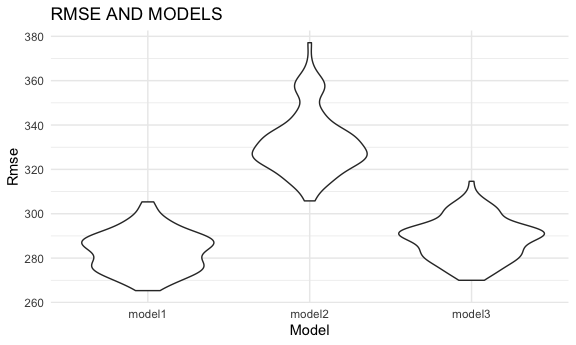
\includegraphics[width=0.9\linewidth]{p8105_hw6_fs2757_files/figure-latex/unnamed-chunk-5-1}

From the plot, the model 2 has the highest prediction error distribution
and the model 1 has the lowest prediction error distribution

\hypertarget{problem-2}{%
\section{Problem 2}\label{problem-2}}

\begin{Shaded}
\begin{Highlighting}[]
\NormalTok{weather\_df }\OtherTok{=} 
\NormalTok{  rnoaa}\SpecialCharTok{::}\FunctionTok{meteo\_pull\_monitors}\NormalTok{(}
    \FunctionTok{c}\NormalTok{(}\StringTok{"USW00094728"}\NormalTok{),}
    \AttributeTok{var =} \FunctionTok{c}\NormalTok{(}\StringTok{"PRCP"}\NormalTok{, }\StringTok{"TMIN"}\NormalTok{, }\StringTok{"TMAX"}\NormalTok{), }
    \AttributeTok{date\_min =} \StringTok{"2017{-}01{-}01"}\NormalTok{,}
    \AttributeTok{date\_max =} \StringTok{"2017{-}12{-}31"}\NormalTok{) }\SpecialCharTok{\%\textgreater{}\%}
  \FunctionTok{mutate}\NormalTok{(}
    \AttributeTok{name =} \FunctionTok{recode}\NormalTok{(id, }\AttributeTok{USW00094728 =} \StringTok{"CentralPark\_NY"}\NormalTok{),}
    \AttributeTok{tmin =}\NormalTok{ tmin }\SpecialCharTok{/} \DecValTok{10}\NormalTok{,}
    \AttributeTok{tmax =}\NormalTok{ tmax }\SpecialCharTok{/} \DecValTok{10}\NormalTok{) }\SpecialCharTok{\%\textgreater{}\%}
  \FunctionTok{select}\NormalTok{(name, id, }\FunctionTok{everything}\NormalTok{())}
\end{Highlighting}
\end{Shaded}

\begin{verbatim}
## Registered S3 method overwritten by 'hoardr':
##   method           from
##   print.cache_info httr
\end{verbatim}

\begin{verbatim}
## using cached file: ~/Library/Caches/R/noaa_ghcnd/USW00094728.dly
\end{verbatim}

\begin{verbatim}
## date created (size, mb): 2021-10-12 10:11:19 (7.604)
\end{verbatim}

\begin{verbatim}
## file min/max dates: 1869-01-01 / 2021-10-31
\end{verbatim}

\begin{Shaded}
\begin{Highlighting}[]
\NormalTok{weather\_df }
\end{Highlighting}
\end{Shaded}

\begin{verbatim}
## # A tibble: 365 x 6
##    name           id          date        prcp  tmax  tmin
##    <chr>          <chr>       <date>     <dbl> <dbl> <dbl>
##  1 CentralPark_NY USW00094728 2017-01-01     0   8.9   4.4
##  2 CentralPark_NY USW00094728 2017-01-02    53   5     2.8
##  3 CentralPark_NY USW00094728 2017-01-03   147   6.1   3.9
##  4 CentralPark_NY USW00094728 2017-01-04     0  11.1   1.1
##  5 CentralPark_NY USW00094728 2017-01-05     0   1.1  -2.7
##  6 CentralPark_NY USW00094728 2017-01-06    13   0.6  -3.8
##  7 CentralPark_NY USW00094728 2017-01-07    81  -3.2  -6.6
##  8 CentralPark_NY USW00094728 2017-01-08     0  -3.8  -8.8
##  9 CentralPark_NY USW00094728 2017-01-09     0  -4.9  -9.9
## 10 CentralPark_NY USW00094728 2017-01-10     0   7.8  -6  
## # ... with 355 more rows
\end{verbatim}

\begin{Shaded}
\begin{Highlighting}[]
\NormalTok{bootstrap\_r }\OtherTok{=}
\NormalTok{  weather\_df }\SpecialCharTok{\%\textgreater{}\%} 
\NormalTok{  modelr}\SpecialCharTok{::}\FunctionTok{bootstrap}\NormalTok{(}\AttributeTok{n =} \DecValTok{5000}\NormalTok{) }\SpecialCharTok{\%\textgreater{}\%} 
  \FunctionTok{mutate}\NormalTok{(}
    \AttributeTok{models =} \FunctionTok{map}\NormalTok{(strap, }\SpecialCharTok{\textasciitilde{}}\FunctionTok{lm}\NormalTok{( tmax }\SpecialCharTok{\textasciitilde{}}\NormalTok{ tmin , }\AttributeTok{data =}\NormalTok{ .x) ),}
    \AttributeTok{results =} \FunctionTok{map}\NormalTok{(models, broom}\SpecialCharTok{::}\NormalTok{glance)) }\SpecialCharTok{\%\textgreater{}\%} 
  \FunctionTok{select}\NormalTok{(.id, results) }\SpecialCharTok{\%\textgreater{}\%} 
  \FunctionTok{unnest}\NormalTok{(results)}

\NormalTok{bootstrap\_r}
\end{Highlighting}
\end{Shaded}

\begin{verbatim}
## # A tibble: 5,000 x 13
##    .id   r.squared adj.r.squared sigma statistic   p.value    df logLik   AIC
##    <chr>     <dbl>         <dbl> <dbl>     <dbl>     <dbl> <dbl>  <dbl> <dbl>
##  1 0001      0.898         0.897  3.08     3185. 8.83e-182     1  -928. 1861.
##  2 0002      0.913         0.913  2.93     3833. 5.33e-195     1  -910. 1825.
##  3 0003      0.902         0.901  2.99     3332. 5.64e-185     1  -917. 1840.
##  4 0004      0.904         0.904  3.08     3410. 1.23e-186     1  -928. 1862.
##  5 0005      0.920         0.920  2.82     4188. 2.07e-201     1  -896. 1798.
##  6 0006      0.904         0.903  3.03     3403. 1.79e-186     1  -921. 1849.
##  7 0007      0.917         0.917  2.89     4023. 1.68e-198     1  -905. 1816.
##  8 0008      0.919         0.919  2.84     4125. 2.65e-200     1  -899. 1803.
##  9 0009      0.915         0.915  2.90     3928. 8.83e-197     1  -905. 1816.
## 10 0010      0.906         0.906  2.96     3508. 1.20e-188     1  -913. 1832.
## # ... with 4,990 more rows, and 4 more variables: BIC <dbl>, deviance <dbl>,
## #   df.residual <int>, nobs <int>
\end{verbatim}

\begin{Shaded}
\begin{Highlighting}[]
\NormalTok{bootstrap\_r }\SpecialCharTok{\%\textgreater{}\%} 
\FunctionTok{ggplot}\NormalTok{(}\FunctionTok{aes}\NormalTok{(}\AttributeTok{x =}\NormalTok{ r.squared)) }\SpecialCharTok{+} 
  \FunctionTok{geom\_density}\NormalTok{() }\SpecialCharTok{+}
   \FunctionTok{labs}\NormalTok{(}
      \AttributeTok{x =} \StringTok{"R squared values"}\NormalTok{,}
      \AttributeTok{y =} \StringTok{"Density"}\NormalTok{,}
      \AttributeTok{title =} \StringTok{"Distribution of R Squared Estimates"}\NormalTok{)}
\end{Highlighting}
\end{Shaded}

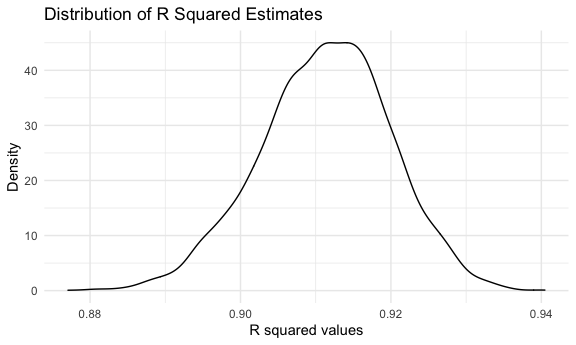
\includegraphics[width=0.9\linewidth]{p8105_hw6_fs2757_files/figure-latex/unnamed-chunk-7-1}

\begin{Shaded}
\begin{Highlighting}[]
\NormalTok{bootstrap\_r}\SpecialCharTok{\%\textgreater{}\%} 
  \FunctionTok{summarize}\NormalTok{(}
    \AttributeTok{CI\_lower =} \FunctionTok{quantile}\NormalTok{(r.squared, }\FloatTok{0.025}\NormalTok{),}
    \AttributeTok{CI\_upper =} \FunctionTok{quantile}\NormalTok{(r.squared, }\FloatTok{0.975}\NormalTok{)}
\NormalTok{  ) }\SpecialCharTok{\%\textgreater{}\%} 
\NormalTok{  knitr}\SpecialCharTok{::}\FunctionTok{kable}\NormalTok{()}
\end{Highlighting}
\end{Shaded}

\begin{longtable}[]{@{}rr@{}}
\toprule
CI\_lower & CI\_upper \\
\midrule
\endhead
0.8936977 & 0.9274807 \\
\bottomrule
\end{longtable}

The plot shows that the R squared estimates appear to be normally
distributed with a mean with 0.911. The 95\% confidence interval for r
squared is (0.8932225, 0.9271586).

\begin{Shaded}
\begin{Highlighting}[]
\NormalTok{bootstrap\_log }\OtherTok{=}
\NormalTok{  weather\_df }\SpecialCharTok{\%\textgreater{}\%} 
\NormalTok{  modelr}\SpecialCharTok{::}\FunctionTok{bootstrap}\NormalTok{(}\AttributeTok{n =} \DecValTok{5000}\NormalTok{)}\SpecialCharTok{\%\textgreater{}\%} 
  \FunctionTok{mutate}\NormalTok{(}
    \AttributeTok{models =} \FunctionTok{map}\NormalTok{(strap, }\SpecialCharTok{\textasciitilde{}}\FunctionTok{lm}\NormalTok{( tmax }\SpecialCharTok{\textasciitilde{}}\NormalTok{ tmin , }\AttributeTok{data =}\NormalTok{ .x) ),}
    \AttributeTok{results =} \FunctionTok{map}\NormalTok{(models, broom}\SpecialCharTok{::}\NormalTok{tidy)) }\SpecialCharTok{\%\textgreater{}\%} 
  \FunctionTok{select}\NormalTok{(.id, results) }\SpecialCharTok{\%\textgreater{}\%} 
  \FunctionTok{unnest}\NormalTok{(results)}\SpecialCharTok{\%\textgreater{}\%} 
  \FunctionTok{select}\NormalTok{(.id, term, estimate) }\SpecialCharTok{\%\textgreater{}\%} 
  \FunctionTok{pivot\_wider}\NormalTok{(}
    \AttributeTok{names\_from =} \StringTok{"term"}\NormalTok{,}
    \AttributeTok{values\_from =} \StringTok{"estimate"}
\NormalTok{  ) }\SpecialCharTok{\%\textgreater{}\%} 
  \FunctionTok{mutate}\NormalTok{(}
    \AttributeTok{log =} \FunctionTok{log}\NormalTok{(}\StringTok{\textasciigrave{}}\AttributeTok{(Intercept)}\StringTok{\textasciigrave{}} \SpecialCharTok{*}\NormalTok{ tmin)}
\NormalTok{  ) }
\NormalTok{bootstrap\_log}
\end{Highlighting}
\end{Shaded}

\begin{verbatim}
## # A tibble: 5,000 x 4
##    .id   `(Intercept)`  tmin   log
##    <chr>         <dbl> <dbl> <dbl>
##  1 0001           7.22  1.04  2.01
##  2 0002           7.17  1.04  2.01
##  3 0003           7.23  1.04  2.02
##  4 0004           7.16  1.03  2.00
##  5 0005           7.39  1.02  2.02
##  6 0006           7.48  1.02  2.03
##  7 0007           7.12  1.06  2.02
##  8 0008           7.26  1.03  2.01
##  9 0009           7.24  1.04  2.02
## 10 0010           7.20  1.05  2.02
## # ... with 4,990 more rows
\end{verbatim}

\begin{Shaded}
\begin{Highlighting}[]
\NormalTok{bootstrap\_log }\SpecialCharTok{\%\textgreater{}\%} 
\FunctionTok{ggplot}\NormalTok{(}\FunctionTok{aes}\NormalTok{(}\AttributeTok{x =}\NormalTok{ log)) }\SpecialCharTok{+} 
  \FunctionTok{geom\_density}\NormalTok{() }\SpecialCharTok{+}
   \FunctionTok{labs}\NormalTok{(}
      \AttributeTok{x =} \StringTok{"Log values"}\NormalTok{,}
      \AttributeTok{y =} \StringTok{"Density"}\NormalTok{,}
      \AttributeTok{title =} \StringTok{"Distribution of log valu"}\NormalTok{)}
\end{Highlighting}
\end{Shaded}

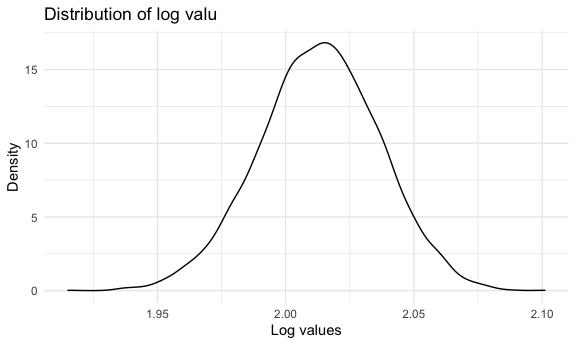
\includegraphics[width=0.9\linewidth]{p8105_hw6_fs2757_files/figure-latex/unnamed-chunk-8-1}

\begin{Shaded}
\begin{Highlighting}[]
\NormalTok{bootstrap\_log}\SpecialCharTok{\%\textgreater{}\%} 
  \FunctionTok{summarize}\NormalTok{(}
    \AttributeTok{CI\_lower =} \FunctionTok{quantile}\NormalTok{(log, }\FloatTok{0.025}\NormalTok{),}
    \AttributeTok{CI\_upper =} \FunctionTok{quantile}\NormalTok{(log, }\FloatTok{0.975}\NormalTok{)}
\NormalTok{  ) }\SpecialCharTok{\%\textgreater{}\%} 
\NormalTok{  knitr}\SpecialCharTok{::}\FunctionTok{kable}\NormalTok{()}
\end{Highlighting}
\end{Shaded}

\begin{longtable}[]{@{}rr@{}}
\toprule
CI\_lower & CI\_upper \\
\midrule
\endhead
1.965633 & 2.058469 \\
\bottomrule
\end{longtable}

The plot shows that the log estimates appear to be normally distributed
with a mean with 2.013 The 95\% confidence interval for r squared is
(1.964318, 2.05832).

\end{document}
